\documentclass[12pt,epsfig]{article}
\usepackage{graphicx,fullpage,url}


\bibliographystyle{unsrt} %for BibTeX - sorted numerical labels by
                          %order of first citation.

\begin{document}

\pagestyle{empty}
\renewcommand{\thefootnote}{\fnsymbol{footnote}}

\begin{flushright}
{\small
Thomas Collins\\
NPG Technote \\ 
2019-TN-02\\
\today\\}
\end{flushright}

\vspace{.5cm}

\begin{center}
Circuit Diagram of DeMeritt 103 and Analysis 
\end{center}
\vspace{.5cm}

\begin{abstract}
Circuit panels are the heart of a houses/rooms electrical system. They control the amount of current provided for each element and whether or not that element is operating. It is important to inspect each element regularly to ensure that it is running within its operational parameters.
\end{abstract}


%\tableofcontents

\section{Motivation}

To analyze each circuit element to ensure that we do not overload it during normal operations or a cooldown. 

\section{Equipment}
This is a list of the equipment you might find useful when analyzing your electrical system 
\begin{enumerate}
\item Ammeter, Voltmeter, and Ohmmeter or a Multimeter to substitute for all three. 
\item Digital Clamp Meter 
\end{enumerate}
 

\section{Analysis}
For the Analysis of DeMeritt 103 I used a Klein Tools Auto-Ranging Digital Clamp Meter

\begin{figure}
\begin{center}
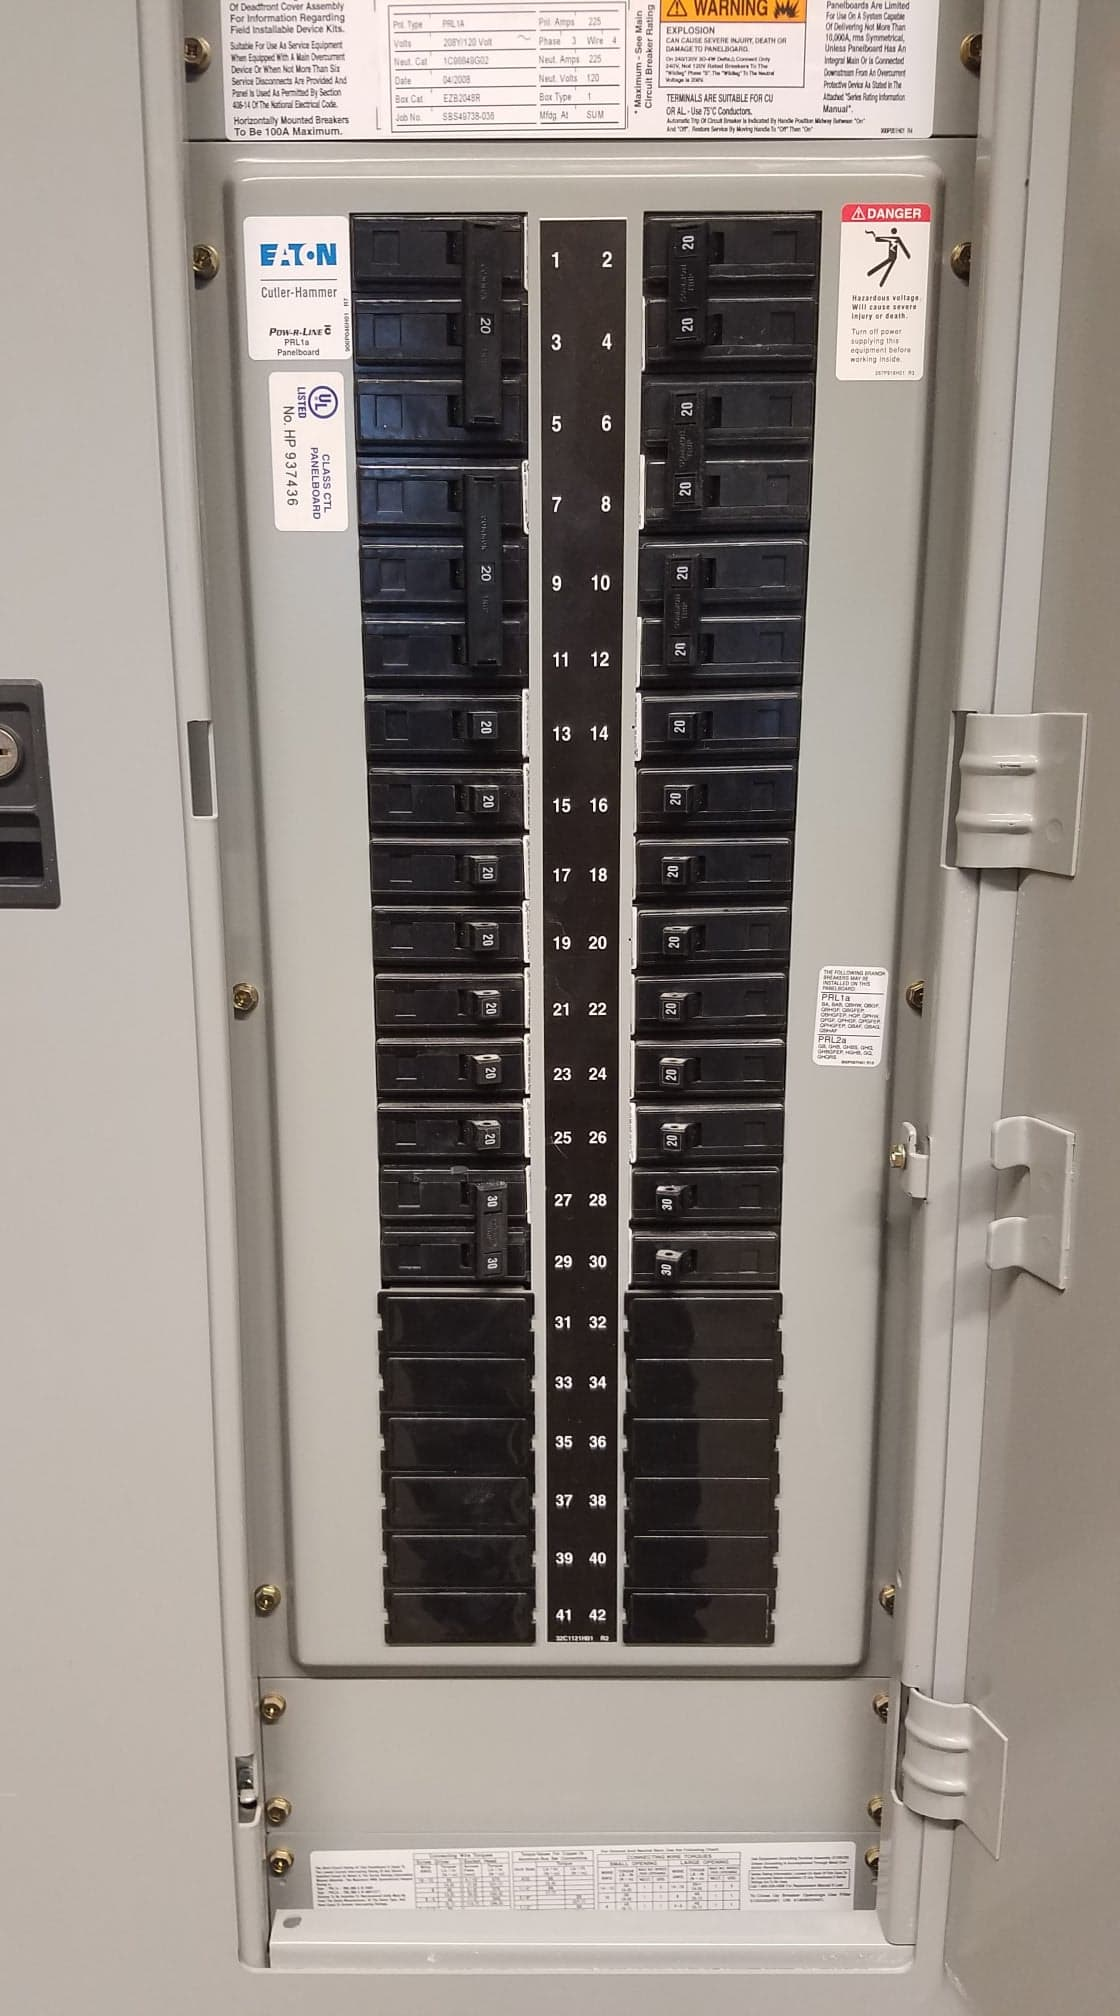
\includegraphics[angle=0,width=0.49\textwidth]{CP}
\caption{\label{ANCHOR} Circuit Panel located on the south wall of DeMeritt 103 }
\end{center}
\end{figure}



\end{document}

